\section{Flujometrías y CFD}
%
Se realizaron una serie de flujometrías para obtener valores de $C_{D}$ en
función de la diferencia de presión a través del puerto y la apertura del
mismo\footnote{ICESym utiliza alzada, por lo que se traduce área de pasaje de
puerto en alzada de válvula equivalente.}, con el fin de obtener un mapa del
coeficiente de descarga en función de la presión y apertura del puerto
($C_{D} = f(\Delta P,l_v)$).
%
ICESym requiere de información del $C_{D}$ para calcular el área efectiva
de pasaje de flujo de las válvulas (o puertos en el caso del MRCVC).
%
Introduciendo el mapa de $C_{D}$ se tiene un mejor modelado del funcionamiento
del sistema de intercambio de gases porque se conoce la pérdida de carga
localizada para un rango de operación del motor.

\nomenclature[PO]{\(\Delta P\)}{Diferencia de Presión entre puerto y cámara}
\nomenclature[PO]{\(l_v\)}{Alzada de válvula o apertura de puerto}

Para las flujometrías se utilizó el software OpenFOAM seleccionando el algoritmo
PIMPLE, con sus implementaciones ``pimpleFoam'' y ``rhoPimpleFoam'' para los
casos en los que se considera un fluido de trabajo incompresible y compresible
respectivamente.
%
La configuración del software se detalla en la Sección~\ref{sec:3_openfoam}.

\subsection{Modelos de Turbulencia}
%
El flujo a través del puerto es de carácter transitorio, turbulento; para
modelar este tipo de flujo se utilizó el modelo de turbulencia de dos ecuaciones
\emph{$\kappa-\epsilon$}\parencite{wilcox}, que consta de una ecuación para la
\emph{energía cinética turbulenta} $\kappa$ y otra para la \emph{tasa de
disipación de la energía cinética turbulenta} $\epsilon$.
%
El modelo está basado en el modelo estándar
$\kappa-\epsilon$~\parencite{launderSpalding} y es uno de los más populares con
\emph{performance} conocida.
%
Las ecuaciones del modelo son:

\begin{equation}\label{eq:k}
  \frac{D}{Dt}(\rho \kappa) = \nabla \cdot (\rho D_{\kappa}\nabla \kappa) + P_{\kappa} - \rho \epsilon
\end{equation}

\nomenclature[PO]{\(\rho\)}{Densidad}
\nomenclature[F]{\(\kappa\)}{Energía cinética turbulenta}
\nomenclature[F]{\(\epsilon\)}{Disipación de energía cinética turbulenta}
\nomenclature[F]{\(D_{\kappa}\)}{Difusividad efectiva para $\kappa$}
\nomenclature[F]{\(P_{\kappa}\)}{Tasa de producción de energía cinética turbulenta}
\nomenclature[F]{\(\epsilon\)}{Tasa de disipación de energía cinética turbulenta}

donde

\begin{itemize}
  \item[-] $\kappa$ es la energía cinética turbulenta.
  \item[-] $D_{\kappa}$ es la difusividad efectiva para $\kappa$.
  \item[-] $P_{\kappa}$ es la tasa de producción de energía cinética turbulenta.
  \item[-] $\epsilon$ es la tasa de disipación de energía cinética turbulenta.
\end{itemize}


\begin{equation}\label{eq:k}
  \frac{D}{Dt}(\rho \epsilon) =
  \nabla \cdot (\rho D_{\epsilon}\nabla \epsilon) +
  \frac{C_{1}\epsilon}{\kappa} \left( P_{\kappa}+C_{3}\frac{2}{3}\kappa\nabla\cdot u \right) -
  C_{2}\rho\frac{\epsilon^{2}}{\kappa}
\end{equation}

donde
\begin{itemize}
  \item[-] $D_{\epsilon}$ es la difusividad efectiva de $\epsilon$.
  \item[-] $C_{1}$ es un coeficiente del modelo.
  \item[-] $C_{2}$ es un coeficiente del modelo.
\end{itemize}

La ecuación para la viscosidad turbulenta $\nu_{t}$ es

\begin{equation}\label{eq:nu_t}
  \nu_{t} = C_{\mu}\frac{\kappa^{2}}{\epsilon}
\end{equation}

\nomenclature[F]{\(\nu_{t}\)}{Viscosidad turbulenta}

donde
\begin{itemize}
        \item[-] $C_{\mu}$ es un coeficiente del modelo.
\end{itemize}

Los coeficientes por defecto del modelo son:

% Clossure Coefficient
\begin{equation}
  C_{\epsilon 1}=1,44
  \quad
  C_{\epsilon 2}=1,92
  \quad
  C_{\mu}=0,09
  \quad
  \sigma_{k}=1
  \quad
  \sigma_{\epsilon}=1,3
\end{equation}

El valor inicial para $\kappa$ se puede estimar con:
\begin{equation}\label{eq:kappa_est}
  \kappa = \frac{3}{2} {\left( |u_{ref}| \cdot I \right)}^{2}
\end{equation}

\nomenclature[F]{\(I\)}{Intensidad de turbulencia}

donde
\begin{itemize}
  \item[-] $I$ es la intensidad de turbulencia en \%.
  \item[-] $u_{ref}$ es una velocidad de referencia en $ms^{-1}$.
\end{itemize}

El valor inicial para $\epsilon$ se puede estimar con:
\begin{equation}\label{eq:epsilon_est}
  \epsilon = \frac{{C_{\mu}}^{3/4} \cdot {\kappa}^{3/2}} {l_{m}}
\end{equation}

donde
\begin{itemize}
 \item[-] $l_{m}$ es una longitud de referencia, para flujos internos se estima
con el diámetro hidráulico de la cañería, usando por ejemplo $0,07 \cdot D_{m}$.
\end{itemize}

\nomenclature[F]{\(l_m\)}{Longitud de mezcla o escala de viscosidad}

% https://www.openfoam.com/documentation/guides/latest/doc/guide-turbulence-ras-k-epsilon.html

Las ecuaciones anteriores de  $\kappa$ y $\epsilon$ son estimaciones para dar un
valor inicial al problema.
%
La longitud de mezcla $l_m$ determina el tamaño que pueden tener los torbellinos
turbulentos, su valor inicial se aproximó como la altura de cámara $l_m = h_c$.
%
Esta estimación de $l_{m}$ a priori parece algo elevado, es un valor que se
utilizó para inicializar la simulación.


\subsection{Condiciones Iniciales}\label{cap2:cond_iniciales}
%
Las condiciones iniciales se determinan para cada diferentes puntos operativos
de interés del motor a partir de los datos obtenidos del simulador ICESym.
%
Se tienen dos casos distintivos al momento de modelar el flujo a través de los
puertos: flujo compresible e incompresible.
%
Para este último se considera que los efectos de la compresibilidad del gas se
pueden despreciar cuando el número de Mach es menor a $0,3-0,4$.
%
Además, se deben separar los casos a modelar entre aquellos en los que hay
solape de cámaras y los que no (ver Figura~\ref{fig:solape}).
%
En estos casos se define también un valor medio para inicializar el interior del
dominio que representa el gas dentro de la cámara de combustión.

\begin{figure}[t!]
  \centering
    \begin{subfigure}[t]{0.4\textwidth}
        \centering
        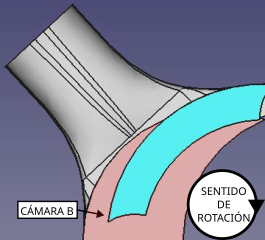
\includegraphics[width=\textwidth]{flujometrias/sin_solape.png}
        \caption{Sin solape}
    \end{subfigure}%
    \begin{subfigure}[t]{0.4\textwidth}
        \centering
        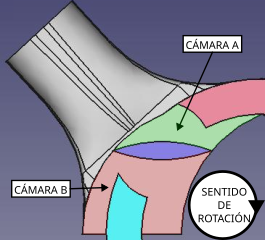
\includegraphics[width=\textwidth]{flujometrias/con_solape.png}
        \caption{Con solape}
    \end{subfigure}
  \caption{Solape de cámaras}\label{fig:solape}
\end{figure}

Independientemente del tipo de flujo que se esté simulando, de ICESym se toman
los valores de presión, temperatura, densidad y velocidad para calcular los
valores iniciales.

Debido a la cantidad de flujometrías a realizar, se utilizó un \emph{script}
para leer los datos de salida de ICESym y calcular los valores requeridos en
función del tipo de flujo a simular.
%
Este \emph{script} toma el estado del gas del simulador tanto en la cámara de
combustión como del puerto que se esté analizando, para la posición de alzada y
RPM requeridas.
%
De la simulación con ICESym se leen los valores listados en la
Tabla~\ref{tab:valores_iniciales} a partir de los cuales se pueden calcular las
propiedades termodinámicas de la mezcla de gases frescos o quemados,
dependiendo si se está evaluando un puerto de admisión o escape.


Para simplificar el análisis no se tuvo en cuenta la fracción de gases
residuales, el gas ``flujado'' es siempre aire limpio en el caso de los puertos
de admisión o el gas quemado de una mezcla estequiométrica de aire-combustible
en caso de los puertos de escape, siendo isooctano $C_{8}H_{18}$ el combustible
seleccionado.
%
Las ecuaciones utilizadas para modelar las propiedades termodinámicas de las
mezclas aire-combustible fueron descritas brevemente en la
sección~\ref{subsec:prop_mezcla}.
%
Los valores calculados son los indicados en la
Tabla~\ref{tab:valores_calculados}.

\begin{table}
  \centering
  \begin{tabular}{cl}\toprule
    Símbolo & Descripción \\ \midrule
    $\rho_{c,i}$ & es la densidad del gas en la cámara $i$ \\
    $P_{c,i}$ & es la presión del gas en la cámara $i$ \\
    $T_{c,i}$ & es la temperatura del gas en la cámara $i$ \\
    $\rho_{p,i}$ & es la densidad del puerto $i$ \\
    $v_{p,i}$ & es la velocidad del gas en el puerto $i$ \\
    $P_{p,i}$ & es la presión del gas en el puerto $i$ \\ \bottomrule
  \end{tabular}
\caption{Valores iniciales}\label{tab:valores_iniciales}
\end{table}

\begin{table}[h]
  \centering
  \begin{tabular}{cll}\toprule
    Símbolo & Descripción & Ecuación\\ \midrule
    $M_{M}$ & masa molar & \ref{eq:mw} \\
    $C_{p}$ & calor específico a presión constante & - \\
    $\gamma$ & relación $C_{p}/C_{v}$ del gas & - \\
    $\mu$ & viscosidad dinámica & \ref{eq:mu} \\
    $\nu$ & viscosidad cinemática & - \\
    $P_{R}$ & número de Prandtl & \ref{eq:pr} \\
    $k_{est}$ & energía cinética turbulenta & \ref{eq:kappa_est} \\
    $\epsilon_{est}$ & disipación de la energía cinética turbulenta & \ref{eq:epsilon_est} \\ \bottomrule
  \end{tabular}
  \caption{Valores calculados}\label{tab:valores_calculados}
\end{table}

\nomenclature[F]{\(M_{M}\)}{Masa molar}
\nomenclature[F]{\(C_{p}\)}{Calor específico a presión constante}
\nomenclature[F]{\(\gamma\)}{Cociente de calores específicos}
\nomenclature[F]{\(\mu\)}{Viscosidad dinámica}
\nomenclature[F]{\(\nu\)}{Viscosidad cinemática}
\nomenclature[F]{\(P_{R}\)}{Número de Prandtl}
\nomenclature[F]{\(k_{est}\)}{Energía cinética turbulenta}
\nomenclature[F]{\(\epsilon_{est}\)}{Disipación de la energía cinética turbulenta}


\subsection{Malla}

La malla se construyó a partir del modelo de CAD generado con los resultados
obtenidos de las simulaciones del motor.
%
La implementación de las diferentes herramientas requeridas para generar una
malla apta para realizar las flujometrías se describe en el
apartado~\ref{sec:cap3_of_malla}.

El grado de refinamiento de la malla utilizada para modelar el dominio de la
flujometría tiene un impacto directo en la calidad de los resultados ya que esta
relacionado con el error de discretización.
%
Por otro lado, mallas con un alto nivel de refinamiento son, en términos de
tiempo más costosas de realizar y dado la cantidad de flujometrías que requiere
el trabajo se optó por determinar un nivel de refinamiento que devuleva un error
relativo entre iteraciones no mayor al $5\%$.

Para los puertos de admisión se seleccionó la geometría representada en la
Figura~\ref{fig:refinamiento_admision}, en esta posición hay dos cámaras de
combustión activas una con el ciclo en $0^{\circ}$ y otra a $120^{\circ}$.
%
Las condiciones iniciales se determinan a partir de datos del simulador con el
motor girando a 2000 RPM.

Para los puertos de escape se seleccionó la geometría representada en la
Figura~\ref{fig:refinamiento_escape}, esta posición corresponde a un período de
solape de los puertos con dos cámaras activas ubicadas en $420^{\circ}$ y
$540^{\circ}$.
%
Las condiciones inciiales se determinan de los datos de ICESym con el motor
girando a 4000 RPM.


Ambos puertos se simularon con tamaños de malla iniciales de 20, 10, 5 y 2,5 mm,
evaluando la variación del caudal con la cantidad de celdas de la malla, ver
Figura~\ref{fig:refinamiento_admision} para el puerto de admisión y
Figuras~\ref{fig:refinamiento_escape} para el puerto de escape.
%
En las Tablas~\ref{tab:convergencia_malla_admision}
y~\ref{tab:convergencia_malla_escape} se presentan los resultados de los
refinamientos junto con el error relativo entre refinamientos sucesivos.

No se observa gran diferencia entre los casos de 20mm a 2,5mm pese a que la
cantidad de celdas es más de 18 veces mayor, esto se debe a que el software
utilizado para realizar el mallado se configuró para realizar un refinamiento de
todas las superficies y bordes, para captar la geometría de los puertos.
%
En la Figura~\ref{fig:conv_malla_admision} o~\ref{fig:conv_malla_escape} se
puede apreciar la diferencia de tamaño entre las celdas cercanas a las paredes
del puerto y las celdas pertenecientes al interior del volumen para la malla con
tamaño inicial de 20mm.

\begin{table}
  \centering
  \begin{tabular}{cccccc}\toprule
    Tamaño de celda & $N^{\circ}$ Celdas & $Q_{0^{\circ}} [dm^{3}/seg]$ & $\varepsilon_{r,0^{\circ}}$ & $Q_{120^{\circ}} [m^{3}/seg]$ & $\varepsilon_{r,120^{\circ}}$ \\ \midrule
    20mm  & 20680  & 16,335 & -        & -22,216 & - \\
    10mm  & 53948  & 15,855 & $3,03\%$ & -22,649 & $1,91\%$ \\
    5mm   & 172853 & 15,58  & $1,76\%$ & -23,323 & $2,89\%$ \\
    2,5mm & 389980 & 15,395 & $1,20\%$ & -23,401 & $0,34\%$ \\ \bottomrule
  \end{tabular}
  \caption{Figura~\ref{fig:conv_malla_admision} tabulada}\label{tab:convergencia_malla_admision}
\end{table}

\begin{table}
  \centering
  \begin{tabular}{cccccc}\toprule
    Tamaño de celda & $N^{\circ}$ Celdas & $\dot{m}_{420^{\circ}} [g/seg]$ & $\varepsilon_{r,420^{\circ}}$ & $\dot{m}_{540^{\circ}} [g/seg]$ & $\varepsilon_{r,540^{\circ}}$ \\ \midrule
    20mm  & 31933  & -78,325 & - & -70,43 & - \\
    10mm  & 83817  & -82,048 & 4,54\% & -75,075 & 6,19\% \\
    5mm   & 234487 & -84,44  & 2,83\% & -78,626 & 4,52\% \\
    2,5mm & 676850 & -83,897 & 0,65\% & -76,766 & 2,42\% \\ \bottomrule
  \end{tabular}
  \caption{Figura~\ref{fig:conv_malla_escape} tabulada}\label{tab:convergencia_malla_escape}
\end{table}

\begin{figure}[ht]
  \centering
  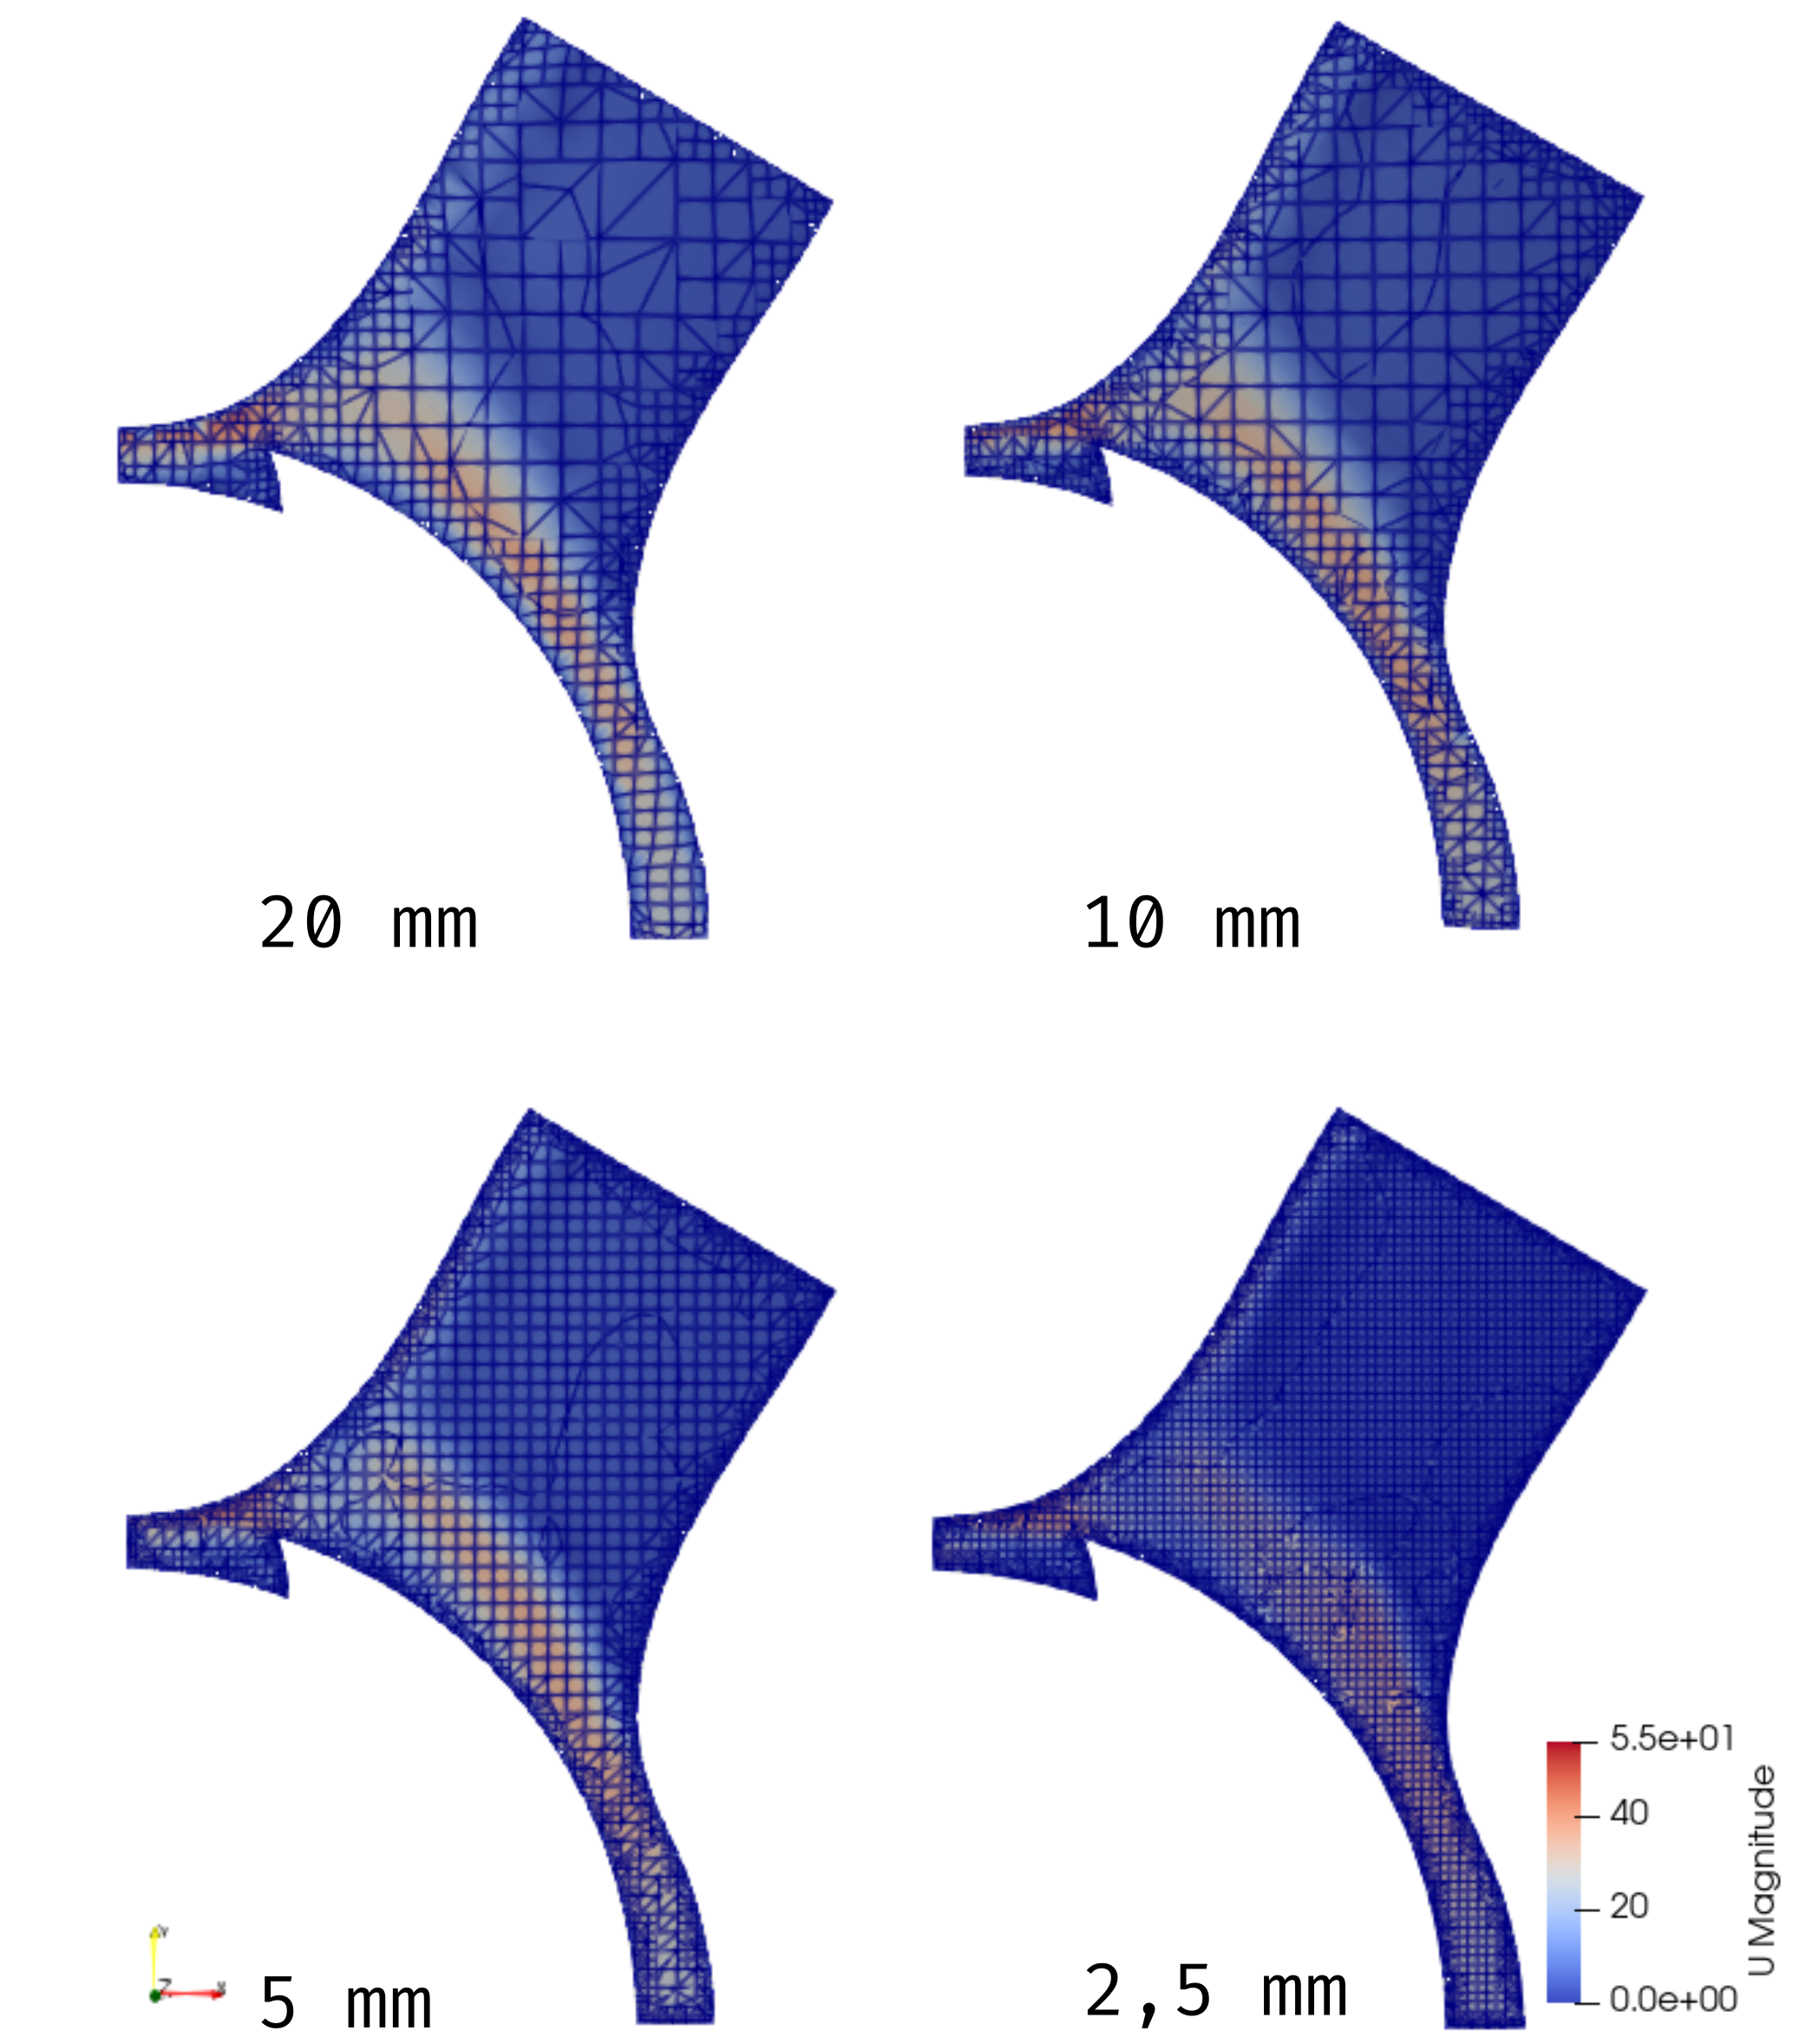
\includegraphics[width=0.8\textwidth]{./flujometrias/refinamiento_malla_admision.png}
  \caption{Refinamiento de malla para puerto de admisión}\label{fig:refinamiento_admision}
\end{figure}

\begin{figure}[ht]
  \centering
  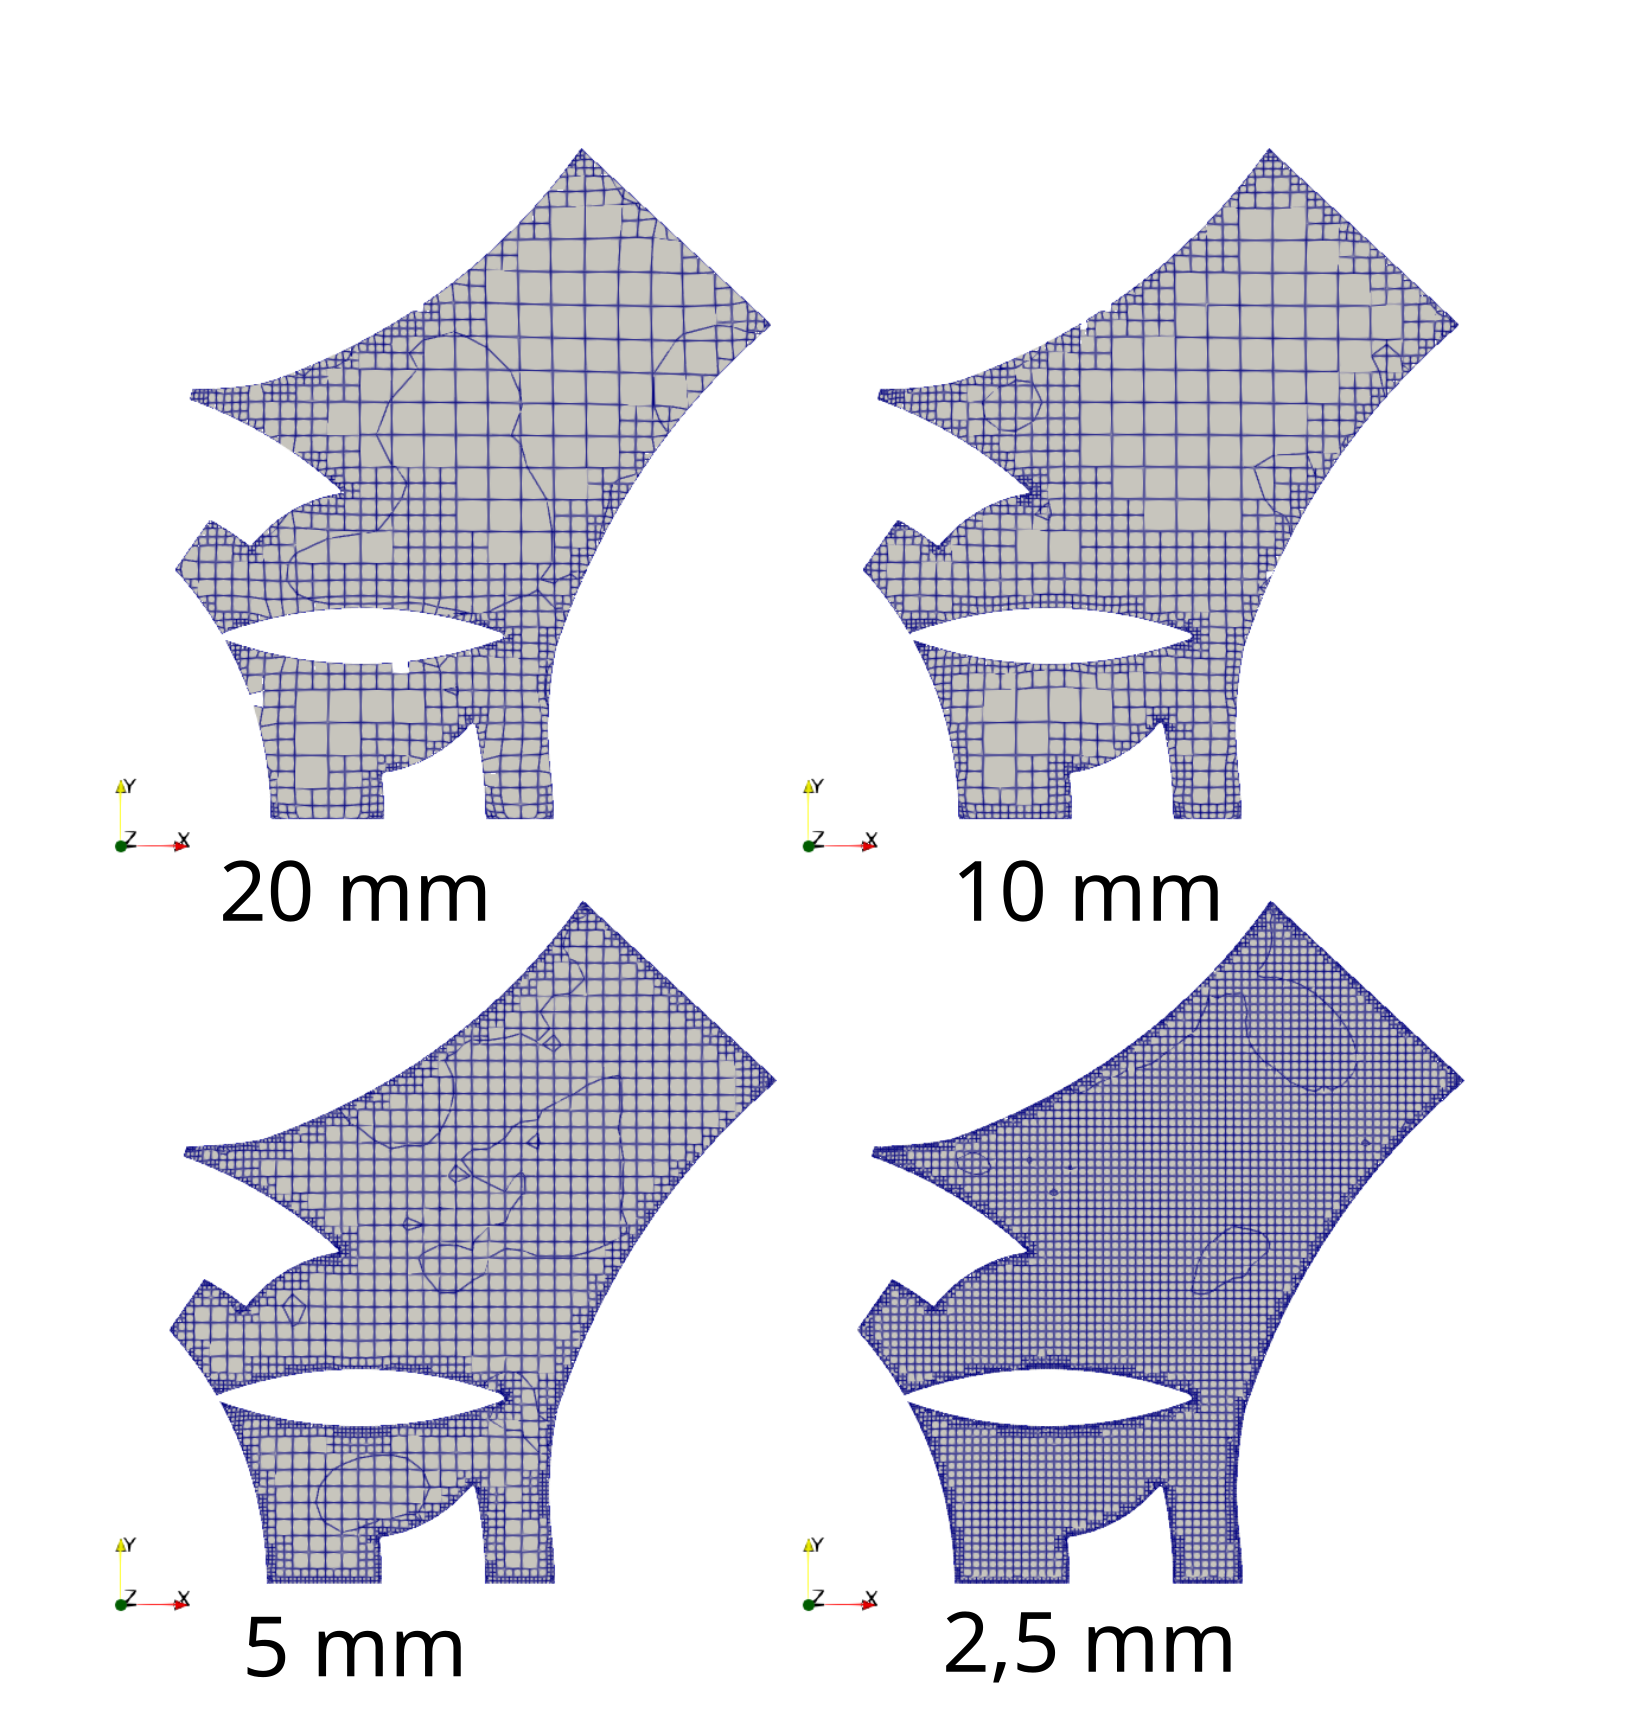
\includegraphics[width=0.8\textwidth]{./flujometrias/refinamiento_malla_escape.png}
  \caption{Refinamiento de malla para puerto de escape}\label{fig:refinamiento_escape}
\end{figure}

\begin{figure}[ht]
  \centering
  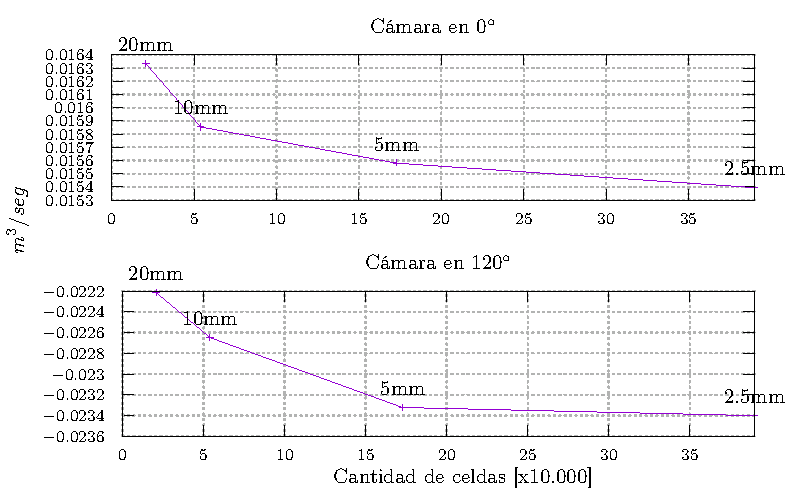
\includegraphics[width=0.9\textwidth]{./flujometrias/convergencia_admision_2000rpm.pdf}
  \caption{Convergencia de malla de puerto de admisión}\label{fig:conv_malla_admision}
\end{figure}

\begin{figure}[ht]
  \centering
  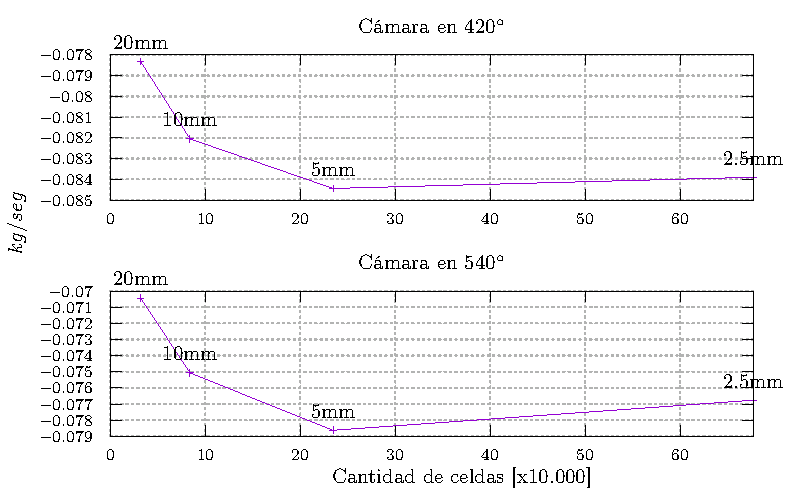
\includegraphics[width=0.9\textwidth]{./flujometrias/convergencia_escape_4000rpm.pdf}
  \caption{Convergencia de malla de puerto de escape}\label{fig:conv_malla_escape}
\end{figure}


\subsection{Coeficiente de Descarga $C_{D}$}\label{sec:cap2_cd}

La pérdida de carga localizada en los puertos de admisión y escape se puede
representar a través del coeficiente de descarga, $C_{D}$.
%
Este coeficiente varía con la geometría y condiciones de operación del puerto,
siendo $C_{D}=1$ el caso ideal sin pérdida de carga localizada.
%
Es un parámetro importante porque permite obtener una mejor estimación del flujo
másico real en el puerto, se define como:

\begin{equation}
  C_{D} = \frac{\text{flujo másico real}}{\text{flujo másico ideal}}
\end{equation}

El $C_{D}$ de un puerto se puede obtener experimentalmente en un banco de prueba
mediante un ensayo que consiste en medir el caudal que circula por un puerto con
una presión de descarga fija que, en equipos comerciales varía entre $250-700$
mm.c.a.
%
Comúnmente estos ensayos se realizan en un banco que incluye solamente la tapa
de cilindros y una camisa que simula el cilindro de la cámara de combustión,
dejando de lado otros elementos del sistema como pistón, los conductos de
admisión y otros.
%
En la imagen~\ref{fig:banco_flujometrias} se muestra un banco de pruebas
comercial.

\begin{figure} \centering
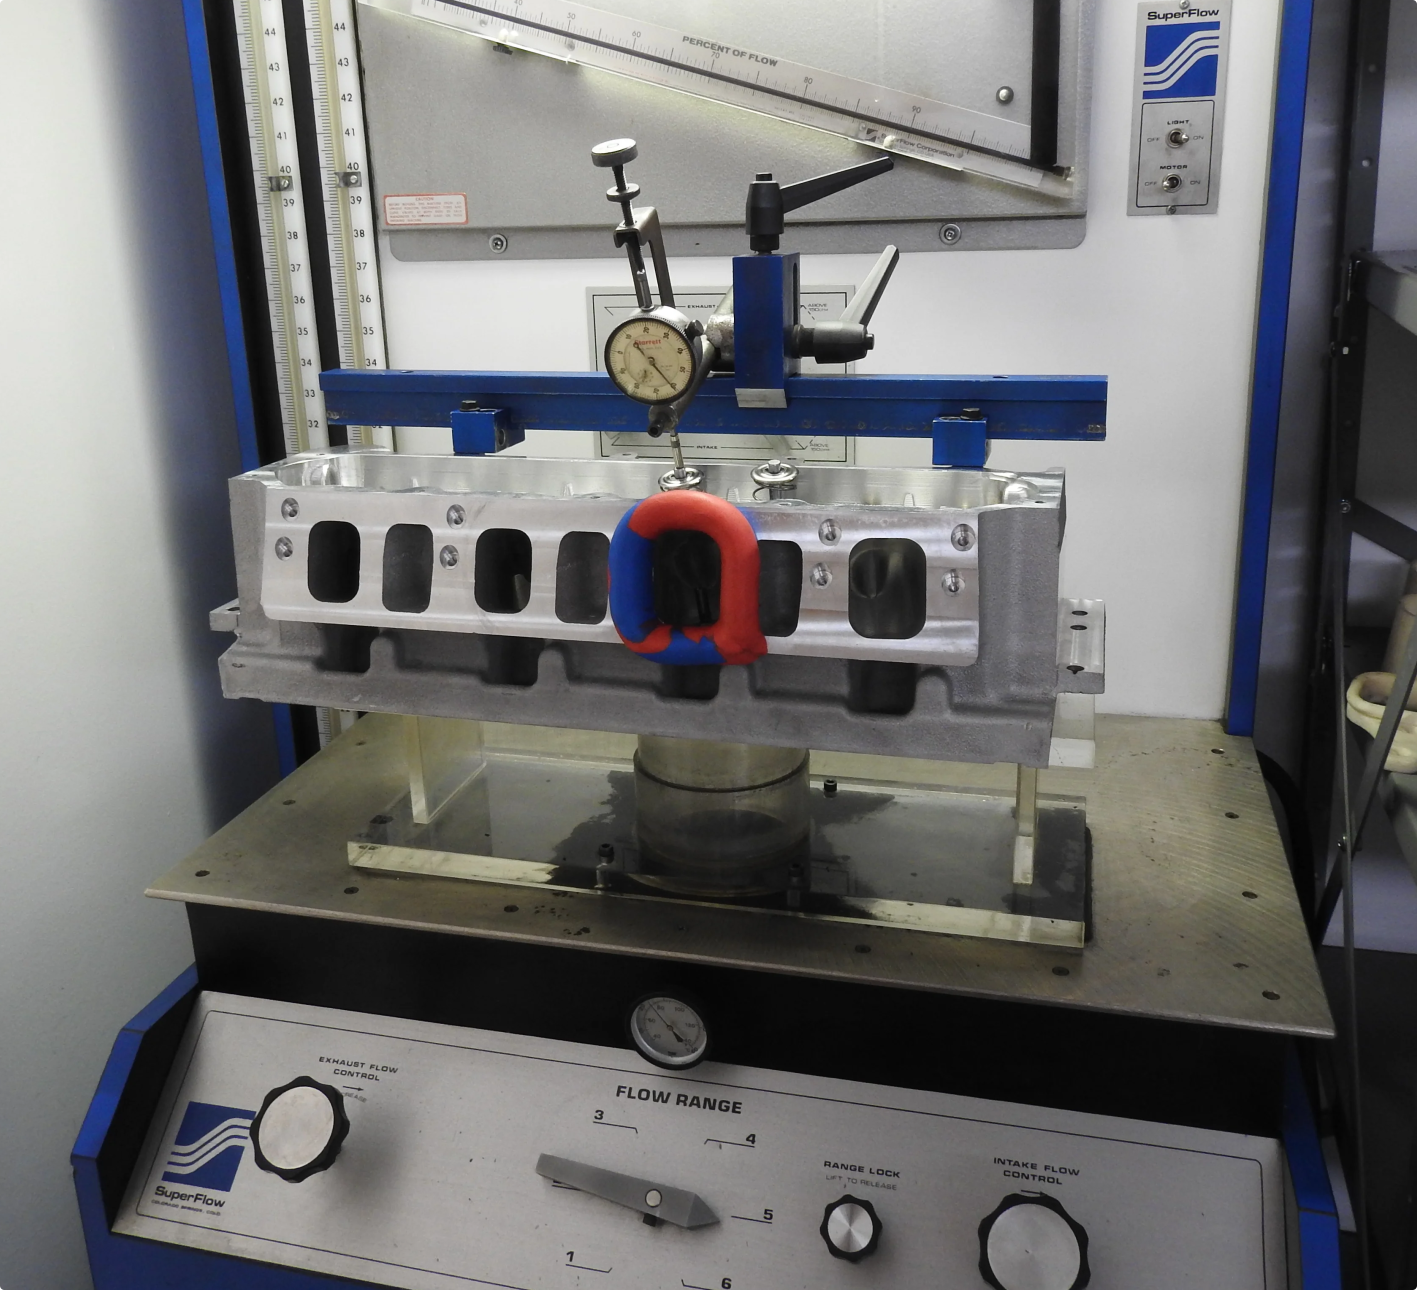
\includegraphics[width=0.7\textwidth]{./flujometrias/banco_flujometrias.png}
  \caption{Banco de flujometrías Super-Flow SF-750}\label{fig:banco_flujometrias}
\end{figure}

Durante el ensayo se mide el caudal de aire atmosférico para diferentes grados
de apertura de la válvula y así se obtienen datos de (alzada, flujo) con los
cuales comparar entre diferentes geometrías del puertos de admisión o escape.
%
En la Figura~\ref{fig:flow-1} se muestra el resultado del ensayo de un
flujómetro en el que se compara la capacidad de flujo de dos tapas de cilindro
diferentes de un BMW S14
\footnote{\url{http://e30sport.net/tech_articles/engine-tech/flow-1/chart-1.htm}}.

\begin{figure} \centering
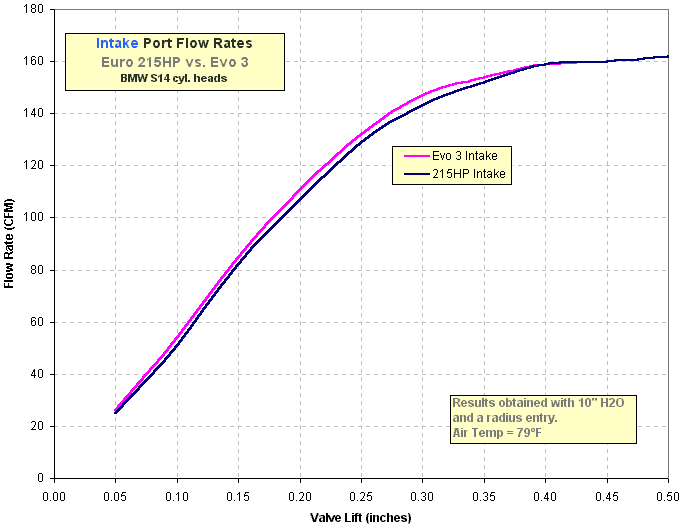
\includegraphics[width=\textwidth]{./flujometrias/flow-1.png}
  \caption{Comparación entre flujometrías de dos tapas de cilindro de un BMW S14}\label{fig:flow-1}
\end{figure}

Otra forma de aproximar un coeficiente de descarga es por medio de flujometrías
computacionales, el uso de CFD permite modelar el puerto en condiciones
operativas, incluyendo la interacción con elementos como por ejemplo el pistón,
o en el caso del MRCVC, estator y conjunto rotante.
%
Además, se puede modelar las propiedades del fluido de trabajo para una
viscosidad, presión y temperatura representativas de las condiciones operativas
del motor que se está modelando.
%
En este trabajo se optó por esta metodología, a partir de las flujometrías se
obtuvo un valor de caudal másico el cual es utilizado para calcular un
coeficiente de descarga.

A partir de $\dot{m}$, el valor de $C_{D}$  se calcula con de las ecuaciones de
flujo compresible a través de una restricción, habiendo dos casos distintivos:
flujo bloqueado y no bloqueado.

Para el caso en que el flujo no esté bloqueado la ecuación de $\dot{m}$ es
la~(\ref{eq:m_no_bloqueado}) y en caso de que se cumpla la
desigualdad~(\ref{eq:cond_bloqueo}) el flujo está bloqueado y se utiliza la
ecuación~(\ref{eq:m_bloqueado}):
%

\begin{equation}\label{eq:m_no_bloqueado}
  \dot{m} = \frac{C_D A_R p_0}{\sqrt{R T_0}} {\left(\frac{p_T}{p_0} \right)}^{1/\gamma} {\left( \frac{2\gamma}{\gamma-1} \left[1- {(\frac{p_T}{p_0})}^{{\gamma-1}/\gamma} \right] \right)}^{1/2}
\end{equation}

\begin{equation}\label{eq:cond_bloqueo}
  \frac{p_T}{p_0} \le {[\frac{2}{\gamma+1}]}^{\gamma/(\gamma - 1)}
\end{equation}

\begin{equation}\label{eq:m_bloqueado}
  \dot{m}=  \frac {C_D A_R p_0} {{(R T_0)}^{1/2}} \gamma^{1/2} {\left( \frac{2\gamma}{\gamma+1} \right)}^{(\gamma+1)/(2(\gamma-1))}
\end{equation}

donde
\begin{itemize}
    \item $p_0$, es la presión de estancamiento antes de la restricción.
    \item $T_0$, es la temperatura de estancamiento antes de la restricción.
    \item $p_T$, es la presión estática justo después de la restricción.
    \item $A_R$, es el área de pasaje de flujo o de referencia.
    \item $\dot{m}$, es el caudal másico.
  \item $\gamma$, es el cociente de capacidades térmicas del gas.
\end{itemize}

\nomenclature[PO]{\(p_0\)}{Presión de estancamiento antes de la restricción}
\nomenclature[PO]{\(T_0\)}{Temperatura de estancamiento antes de la restricción}
\nomenclature[PO]{\(p_T\)}{Presión estática justo después de la restricción}
\nomenclature[G]{\(A_R\)}{Área de pasaje de flujo o de referencia}

El flujo está bloqueado si la velocidad en la garganta de la restricción alcanza
la velocidad sónica, dada esta condición $\dot{m}$ alcanza un límite y reducir
la presión aguas abajo de la restricción no produce un aumento del caudal.
%
% La condición de flujo bloqueado se puede expresar en términos de la relación de
% presiones aguas arriba $p_{0}$ y aguas abajo de la restricción $p_{T}$.
%
Las presiones y temperaturas involucradas en el cálculo de $\dot{m}$ se pueden
medir u obtener de una simulación computacional del ciclo del motor.
%
\nomenclature[PO]{\(p,P\)}{Presión}

Un parámetro importante en las ecuaciones utilizadas para el cálculo del
coeficiente de descarga $C_{D}$ es el área de referencia $A_{R}$ que define el
área utilizada para calcular el caudal másico que circula por el puerto.
%
% En un motor con válvulas se suele tomar el área de cortina como el producto de
% la circunferencia de la válvula con la alzada, es decir:

La elección del área de referencia utilizada para el cálculo es arbitraria, sin
embargo en un motor con válvulas se suele utilizar el área de cortina (ver
Figura~\ref{fig:area_cortina}) la cual es el producto de la circunferencia y la
alzada de válvula.

\begin{equation} \label{eq:area_cortina}
  A_R = A_C = \pi D_v l_v
\end{equation}

\nomenclature[G]{\(A_R\)}{Área de pasaje de flujo o de referencia}
\nomenclature[G]{\(A_C\)}{Área de cortina}
\nomenclature[G]{\(D_v\)}{Diámetro de válvula}
\nomenclature[G]{\(l_v\)}{Alzada de válvula}

\begin{figure} \centering
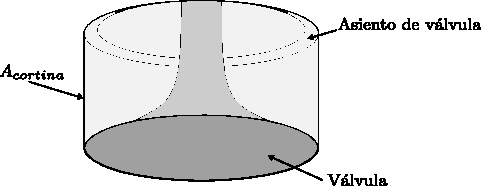
\includegraphics[width=0.5\textwidth]{valve_curtain.pdf}
  \caption{Área de cortina}\label{fig:area_cortina}
\end{figure}

El área de referencia utilizada en ICESym es el área frontal del puerto expuesta
a la cámara que se esté analizando, calculada como:

\begin{equation}\label{eq:ar_mrcvc}
  A_{R,i} = h_{p} \cdot l_{v,i}
\end{equation}

El área de cortina se ilustra en la Figura~\ref{fig:area_cortina} y el área
utilizada en ICESym para el MRCVC en la Figura~\ref{fig:area_referencia}.
%
En esta última figura se observan dos zonas coloreadas, que hacen referencia al
área de dos cámaras durante el solape que ocurre por la geometría del motor.

\begin{figure}
  \centering
  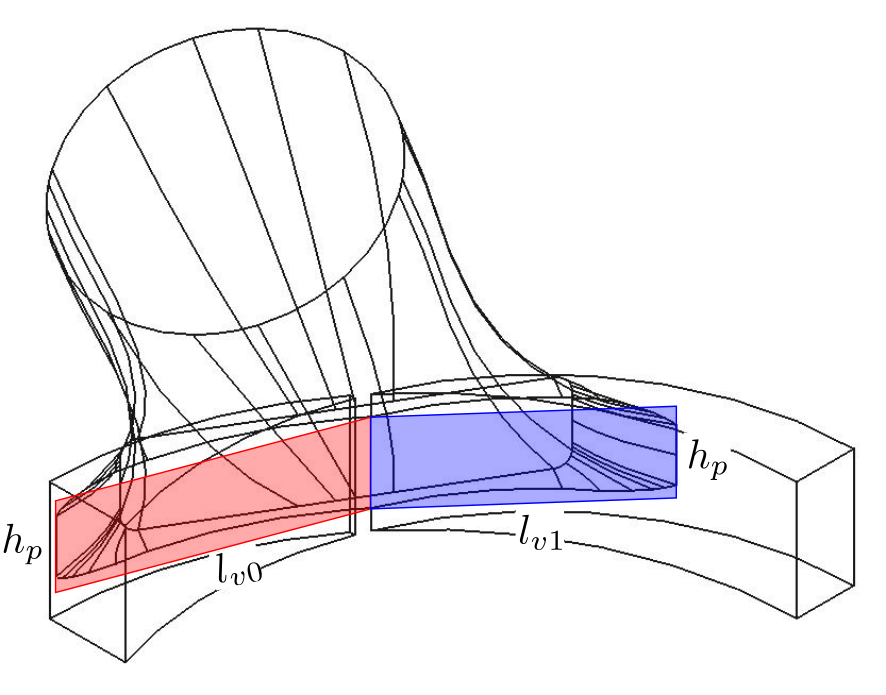
\includegraphics[width=.7\textwidth]{area_referencia.png}
  \caption{Área de referencia MRCVC}\label{fig:area_referencia}
\end{figure}

Los valores de densidad, velocidad, presión y temperatura se obtienen de los
datos de salida de ICESym para un puerto, ángulo y velocidad dada.
%
Para la temperatura se utiliza la temperatura de la cámara, $T_0 = T_C$, la
presión antes y después del puerto se selecciona de acuerdo al sentido de flujo,
en caso de ser hacia la cámara de combustión la presión en el puerto se utiliza
como inicial $P_0$ y la presión en la cámara es la aproximación a la presión en
la restricción $P_T$.
\nomenclature[PO]{\(T\)}{Temperatura}
\nomenclature[SU]{\(0\)}{Valor inicial}

El valor de $\gamma$ se obtiene de las propiedades de la mezcla con las rutinas
computacionales descritas en el apartado~\ref{subsec:prop_mezcla}.

\subsection{Esquemas de Discretización}

Se utilizan para resolver ecuaciones de variables continuas con funciones
discretas en tiempo y espacio.
%
Se deben seleccionar esquemas para resolver:

\begin{itemize}
  \item Primera derivada temporal
  \item Interpolación
  \item Gradiente
  \item Divergencia
  \item Gradientes normales a superficies
  \item Laplacianos
\end{itemize}


\paragraph{Derivadas temporales, $\delta / \delta t$}
%
Estas derivadas se discretizan con el método de Euler\parencite{burden}, que
aproxima la integración de un paso $n$ a $n+1$ con $y_{n+1}-y_{n}\simeq hf_{n}$
donde $h = t_{n+1}-t_{n}$ es el paso temporal y $f_{n}=f(t_{n},y_{n})$.
%
Para el esquema de Euler hacia atrás la aproximación es
$y_{n+1}-y_{n}\simeq h f_{n+1}$.
%
A este esquema se le agrega un coeficiente $\gamma\in[0,1]$ de modo que:

\begin{equation}
  y_{n+1}-y_{n} \simeq \gamma h f_{n+q} + (1-\gamma)h f_{n}
\end{equation}

Con $\gamma=1/2$ el esquema es equivalente a Crank-Nicolson estándar, se puede
convertir al esquema de Euler hacia adelante con $\gamma=0$.

\paragraph{Gradientes}
%
Se discretiza utilizando integración Gaussiana con interpolación lineal entre
valores de celdas.
%
El método define al gradiente medio en un elemento de volumen finito con
centroide \textbf{C} y volumen $V_{c}$ en términos de los flujos a través de sus
caras, como lo indica la ecuación~(\ref{eq:green_gauss_gradient}).
%
Para esto se requiere conocer los valores de la variable $\phi_{f}$ en las caras
vecinas e información del área de la celda y su normal $(\vec{S}_{f})$.

\begin{equation}
  \label{eq:green_gauss_gradient}
  \nabla \phi_{P} = \frac{1}{V_{c}}\sum_{f} \vec{S}_{f}\phi_{f}
\end{equation}

El método de volúmenes finitos utiliza valores en las caras de las celdas, por
lo que se debe aproximar el valor de la variable en una cara dada para obtener
el valor del gradiente en dicha celda.
%
Los valores de $\phi_{f}$ se obtienen de una interpolación lineal entre valores
conocidos de celdas adyacentes.
%
Un método de interpolación entre celdas puede ser:

\begin{align}
  \label{eq:interpolacion_lineal_caras}
  \alpha &= \frac{|{\vec{r}_{N}-\vec{r}_{f}}|} {|{\vec{r}_{N}-\vec{r}_{P}}|}\\
  \phi_{f} &= \alpha\phi_{P}+(1-\alpha)\phi_{N} \\
\end{align}

Donde $\alpha$ es un factor de ponderación geométrico entre las celdas \textbf{P} y
\textbf{N} y $\vec{r}$ es un vector de posición.

La interpolación se puede limitar para que los valores obtenidos se encuentren
entre el mínimo y máximo de las celdas vecinas, este método se denomina
``limitado''.


%Gradiente normal a la superficie
\paragraph{Gradiente normal a una superficie}
%
Este gradiente es evaluado en la cara de la celda.
%
Es la componente (normal a la cara) del gradiente entre los valores de los
centroides de 2 celdas conectadas por la cara evaluada.
%
En general las mallas utilizadas para modelar geometrías reales no son
ortogonales.
%
Esto hace que un vector $S_{f}$ normal a una superficie no necesariamente sea
colineal con el vector que une el centroide de dos celdas contiguas.
%
El gradiente en la cara en la dirección que une los centroides (C y F) de las
celdas $\vec{e}$ es

\begin{equation}
  \label{eq:gradiente_normal}
  (\nabla \phi \cdot \vec{e_{f}}) = \frac{\nabla\phi}{\delta n} = \frac{\phi_{F} - \phi_{C}}{||\vec{r_{C}}-\vec{r_{F}}||} = \frac{\phi_{F} - \phi_{C}}{d_{CF}}
\end{equation}

Donde el subíndice \textbf{f} indica que se evalúa en la cara de una celda.
%
El vector de superficie $S_{f}$ se puede escribir en términos de sus componentes
normal y tangente a la cara $f$ en la que es evaluado.

\begin{equation}
  \vec{S_{f}}= \vec{E_{f}} + \vec{T_{f}}
\end{equation}

De esta forma, el gradiente del flujo de la variable $\phi$ en mallas no
ortogonales se puede expresar en términos de las componentes normal y tangente a
la cara de la celda~\parencite{moukalled}.
%
El término \textbf{E} indica el flujo de $\phi$ normal a la cara y \textbf{T} el
flujo tangente.

\begin{align}
  \label{eq:gradiente}
  %
  {(\nabla \phi)}_{f}\cdot \vec{S_{f}} &= {(\nabla \phi)}_{f}\cdot E_{f} + {(\nabla \phi)}_{f}\cdot \vec{T_{f}} \\
  %
  &= \vec{E_{f}}\frac{\phi_{F}-\phi_{C}}{d_{FC}}+ {(\nabla \phi)}_{f}\cdot \vec{T_{f}}
\end{align}

%
Algunos esquemas de discretización de este tipo de gradientes son:
\begin{itemize}
  \item No corregido
  \item Ortogonal
  \item Corregido y limitado
\end{itemize}

La corrección ortogonal rota el vector $S_{f}$ hasta que sea normal a la superficie.
%
La corrección limitada aplica la corrección ortogonal, sumando
$\cos^{-1}{\theta}$, donde $\theta$ es el ángulo entre la normal a la cara y el
vector $S_{f}$.

% Divergencia
\paragraph{Divergencia}
%
Se utiliza un esquema de integración Gaussiana con interpolación lineal para
la discretización de la divergencia.

Dependiendo de los tipos de variable, se utilizan diferentes esquemas de
interpolación disponibles son:
%
\begin{itemize}
        \item centrada
        \item hacia adelante
        \item hacia atrás
        \item limitada
\end{itemize}

\paragraph{Laplacianos}
%
Los términos Laplacianos se discretizan utilizando integración Gaussiana con
interpolación lineal.


\subsubsection{Resumen de Esquemas Seleccionados}
%
Los esquemas de discretización utilizados fueron, para el caso de \textbf{flujo
incompresible}:

\begin{itemize}
  \item Tiempo: Euler hacia atrás
  \item Gradiente:
        \begin{itemize}
                \item $\nabla p$: Integración Gaussiana con interpolación lineal
                \item $\nabla U$: Integración Gaussiana con interpolación lineal
        \end{itemize}
  \item Divergencia:
        \begin{itemize}
                \item $\nabla\cdot (\phi U)$: Integración Gaussiana con interpolación lineal de segundo orden, hacia adelante limitada con $\nabla U$
                \item $\nabla\cdot (\phi k)$: Integración Gaussiana con interpolación lineal hacia adelante
                \item $\nabla\cdot (\phi \epsilon)$: Integración Gaussiana hacia adelante con interpolación lineal
                \item $\nabla\cdot (\phi R)$: Integración Gaussiana con interpolación lineal
                \item $\nabla\cdot R$: Integración Gaussiana con interpolación lineal
                \item $\nabla\cdot \nu_{eff}$: Integración Gaussiana con interpolación lineal

        \end{itemize}
  \item Laplacianos: Integración Gaussiana con interpolación lineal
  \item Interpolación: Lineal
  \item Gradientes normales a la superficie: sin corregir
\end{itemize}

Donde $\phi$ es el flujo volumétrico en la cara de la celda.
%
Para los casos de \textbf{flujo compresible}:

\begin{itemize}
        \item Esquemas temporales: Euler
        \item Gradientes: Integración Gaussiana con interpolación lineal limitada por las celdas.
        \item Divergencia:
        \begin{itemize}
                \item $\nabla \cdot (\phi U)$: Integración Gaussiana con interpolación lineal de segundo orden, hacia adelante limitada con $\nabla U$
                \item $\nabla \cdot (\phi,e)$: Integración Gaussiana con interpolación lineal limitada
                \item $\nabla \cdot (\phi,h)$: Integración Gaussiana con interpolación linear hacia adelante
                \item $\nabla \cdot (\phi,p)$: Integración Gaussiana con interpolación lineal limitada
                \item $\nabla \cdot (\phi,K)$: Integración Gaussiana con interpolación lineal
                \item $\nabla \cdot (\phi,p)$: Integración Gaussiana con interpolación lineal limitada
                \item $\nabla \cdot (\phi,k)$: Integración Gaussiana con interpolación lineal
                \item $\nabla \cdot (\phi,\epsilon)$: Integración Gaussiana con interpolación lineanl hacia adelante
                \item $\nabla \cdot (((\rho\cdot \nu_{Eff}) dev2((\nabla U)^{T})))$ Integración Gaussiana con interpolación lineal
        \end{itemize}
        \item Laplacianos: Integración Gaussiana con interpolación lineal, limitada y corregida
        \item Interpolación: lineal
        \item Gradientes normales a la superficie: corregida
\end{itemize}

Donde $\phi$ es el flujo másico en la cara de la celda.

